\chapter{Estatística}

\section{Medidas de Tendência Central}

\subsection{Média Aritmética}

\quest{Oficial de Justiça 2023 - VUNESP}{O gráfico apresenta o número de acertos na prova de Língua Portuguesa e de Matemática, aplicada a dois candidatos, A e B, em um concurso interno para promoção de cargo:\\
	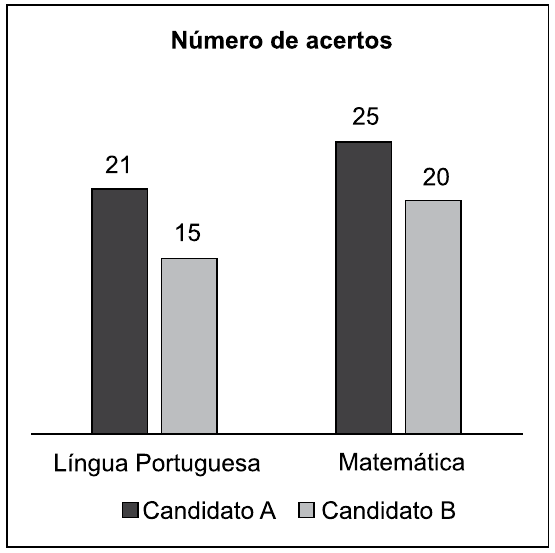
\includegraphics[scale=.5]{fig001.png}\\
Sabendo-se que a prova de Língua Portuguesa tinha 	peso 2 e a de Matemática tinha peso 3 para o cargo em 	concurso, que cada uma das provas tinha 50 questões, 	e que a nota de cada prova é igual ao número de acertos correspondente, é correto afirmar que o número de questões de Matemática que o candidato B deveria ter acertado a mais, para que a média aritmética ponderada das notas das suas provas fosse igual à média aritmética ponderada das notas das provas do candidato A, é igual a}
{\item 9.
\item 20.
\item 10.
\item 29.
\item 27.}
{https://youtu.be/BvsQZctqarQ}

\quest{Guarda Metropolitano Prefeitura de Palmas TO - VUNESP 2023
}{Um motorista de táxi cobra o preço fixo de R\$ 140,00 por corrida até o aeroporto. A tabela mostra algumas informações sobre o número dessas corridas feitas em cinco semanas.
\begin{center}
\begin{tabular}{c|c}
\hline 
\rule[-1ex]{0pt}{2.5ex} Semana & Nº de corridas \\ 
\hline 
\rule[-1ex]{0pt}{2.5ex} 1ª & 3 \\ 
\hline 
\rule[-1ex]{0pt}{2.5ex} 2ª & 5 \\ 
\hline 
\rule[-1ex]{0pt}{2.5ex} 3ª & x \\ 
\hline 
\rule[-1ex]{0pt}{2.5ex} 4ª & x+1 \\ 
\hline 
\rule[-1ex]{0pt}{2.5ex} 5ª & 4 \\ 
\hline 
\end{tabular} 
\end{center}
Sabendo que, na média, foram feitas cinco corridas por semana até o aeroporto, então, a diferença entre a semana em que ele mais arrecadou e a semana em que ele menos arrecadou foi}{
\item R\$ 280,00.
\item R\$ 420,00.
\item R\$ 560,00.
\item R\$ 700,00.}
{https://youtu.be/iYMMAQnHO5A}

\section{Medidas de Dispersão}
\subsection{Desvio Padrão}

\quest{Transpetro 2023 - CESGRANRIO}
{Uma empresa, em reconhecimento ao desempenho de 10 de seus funcionários, decide dar-lhes um bônus. Para tanto, a empresa distribuiu um total de R\$ 25.000,00, de acordo com a Tabela a seguir:
\begin{center}
\begin{tabular}{c|c}
\hline 
Número de   & Valor do Bônus\\ 
funcionários & (em reais) \\ 
\hline
6 & 2000 \\ 
\hline 
2 & 2500 \\ 
\hline 
2 & 4000 \\ 
\hline 
\end{tabular} 
\end{center}
Nessas condições, o desvio padrão dos bônus pagos é dado por}
{
\item $\sqrt{\dfrac{36 \cdot 2000^2 + 4\cdot 2500^2 + 4\cdot 4000^2}{10}}$
\item $\sqrt{\dfrac{36 \cdot 500^2 + 4\cdot 2500^2 + 4\cdot 1500^2}{10}}$
\item $\sqrt{\dfrac{6 \cdot 2000^2 + 2\cdot 2500^2 + 2\cdot 4000^2}{10}}$
\item $\sqrt{\dfrac{500^2 + 1500^2}{10}}$
\item $\sqrt{\dfrac{6 \cdot 500^2 + 2\cdot 1500^2}{10}}$
}
{https://youtu.be/fDPDxc8zjzY}

\quest{Transpetro 2023 - CESGRANRIO}
{Em uma escola, há cinco turmas que fizeram uma prova de matemática, e cada uma possui 60 estudantes. As notas obtidas em cada turma tiveram as seguintes distribuições:
\begin{itemize}
\item Turma 1: 30 notas iguais a 0 e 30 notas iguais a 10;
\item Turma 2: 30 notas iguais a 2 e 30 notas iguais a 8;
\item Turma 3: 30 notas iguais a 3 e 30 notas iguais a 7;
\item Turma 4: 30 notas iguais a 4 e 30 notas iguais a 6;
\item Turma 5: 60 notas iguais a 5.
\end{itemize}
Em qual das turmas o desvio-padrão das notas obtidas foi igual a zero?}
{
\item Turma 1
\item Turma 2
\item Turma 3
\item Turma 4
\item Turma 5}
{https://youtu.be/KkKYd_ILgn8}